\section{Manuel Technique}

Dans cette partie, sera expliqué le fonctionnement de chaque application, en particulier, le framework développé pour la smartforce.

Le but est de fournir assez d'information afin de faciliter le maintient et la manipulation des applications développées.

	\subsection{EternityII (bruteforce)}
	
Cette application a été bâtie de façon à pouvoir rapidement intégrer de nouvelles méthodes de parcours. Elle intègre aussi différents outils de manipulation de fichiers.

Son fonctionnement est simple. Chaque classe accomplit une certaine tâche spécifique \autocite{wiki:kissprinciple}.

D'abord, on charge le fichier d'instance (main.cpp) grâce à la classe \lstinline[language=c++]|FileIn|. 

Une fois les données récupérés du fichier, le \lstinline[language=c++]|Jeu| est initialisé (les différentes \lstinline[language=c++]|Pieces| ainsi que le plateau).

Le jeu est ensuite envoyé à \lstinline[language=c++]|Generator| qui va initialiser les données nécessaires à la résolution. 

Grâce à la fonction  \lstinline[language=c++]|Genetrator::multipleGeneration| ou directement  \lstinline[language=c++]|G::parcoursBruteforce|, on définit le type de parcours. En fonction du type de parcours, le chemin est initialisé par  \lstinline[language=c++]|G::coordinatesCreator|. 

Une fois le chemin sur le plateau initialisé (voir \autoref{fig:parcours_rowscan}), le solveur (\lstinline[language=c++]|G::generationRecursive|) est lancé . Celui-ci va, en fonction des coordonnées, tester si les pièces peuvent être placés (les pièces de coins ne seront testés que sur les coins, \dots). 

Lorsqu'une solution est trouvée, l'évenement \lstinline[language=c++]|G::solutionFoundEvent| est déclenché. 

	\subsection{EternityII--corolle\_generator}
	
Le générateur de corolle est directement inspiré de l'application de bruteforce. Au lieu de résoudre tout le plateau, il résout une sous-partie de celui-ci (une corolle).

Lorsqu'une corolle est trouvée, au lieu de déclencher l'évènement, il va copier les pièces dans un objet \lstinline[language=c++]|Corolle|, la frontière de la corolles est aussi déterminée à ce stade. La corolle et la frontière sont envoyés à la fonction \lstinline[language=c++]|Generator::writeInFile|.

Si un fichier est déjà ouvert, celle-ci vérifie si ces données sont identiques:

\begin{itemize}
	\item si la taille du plateau est identique
	\item le hamming de la corolle
	\item la pièce centrale (et son orientation) 
	\item la zone de la corolle (représentée sous forme de coordonnées $(x,y)$)
\end{itemize}
	
	Si aucun fichier n'est ouvert ou que l'une de ces données est différente, un nouvel objet \lstinline[language=c++]|FileOut| est créé et remplace le précédent.
	
	\lstinline[language=c++]|FileOut| va alors créer ou ouvrir (en supprimant le contenu) le fichier et écrire 4 lignes contenant toutes les informations de la corolle. 
	
	Les deux premières lignes sont sous cette forme :
	
	\begin{exmp}\ 
		
		\begin{lstlisting}[language=bash]
# taille rotation_corolle no_piece rotation x y hamming nb_pieces
# 6 0 0 0 0 0 1 3
	\end{lstlisting}
	\end{exmp}
	
	Sera ensuite écrit la ligne contenant les information de la corolle :
	
	\begin{exmp}
		\lstinline[language=bash]{0:0;5:1;6:0;;|3;4;5;6;7;;;;;;;0}
	\end{exmp}
	
	Si les données du fichier sont identiques, alors la corolle est ajoutée au fichier grâce à la fonction \lstinline[language=c++]{FileOut::put}.
	
	\subsection{EternityII--cardinality\_counter} 
	
On parcours d'abord le fichier contenant les corolles (\lstinline[language=python]|count()|) comptant le nombre de pièces uniques à chaque position (\lstinline[language=python]|count_pieces()|).

Vient ensuite \lstinline[language=python]|put_on_plate()| qui se charge de convertir chaque position en coordonnées $(x,y)$ et en y mettant le nombre d'occurences.

Enfin \lstinline[language=python]|display_plate()| qui affiche ou enregistre, en fonction des options, le plateau avec les occurences.

	\subsection{EternityII--corolle\_rotator}
	
Lorsqu'une corolle est tournée, non seulement les pièces sont tournées, mais l'ordre de parcours change aussi (voir \autoref{fig:corolle_zone_orientee} et \autoref{fig:corolle}). Par conséquent, il suffit non seulement de tourner les pièces \lstinline[language=python]|pieces_rotate()| mais aussi de \enquote{shifter} les pièces.

\begin{exmp}
	Prenons une corolle en $(1,1)$ (Z5 dans la \autoref{fig:corolle_zones_h_1}).
	on obtient donc : \\
	\begin{minipage}{0.24\textwidth}
		\begin{figure}[H]
			\centering
			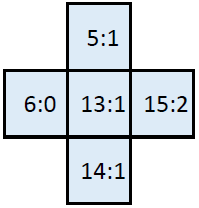
\includegraphics[width=\linewidth]{images/corolle_ex_orientee}
			\caption{Exemple de corolle de hamming 1 en $(1,1)$}
			\label{fig:corolle_ex_orientee}
		\end{figure}
	\end{minipage}\hfill
	\begin{minipage}{0.24\textwidth}
		\begin{figure}[H]
			\centering
			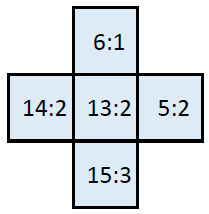
\includegraphics[width=\linewidth]{images/corolle_ex_orientee_1}
			\caption{Exemple de corolle de hamming 1 en $(5,1)$ }
			\label{fig:corolle_ex_orientee_1}
		\end{figure}
	\end{minipage}\hfill
	\begin{minipage}{0.24\textwidth}
		\begin{figure}[H]
			\centering
			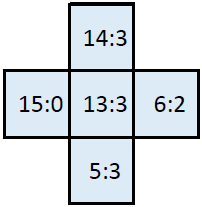
\includegraphics[width=\linewidth]{images/corolle_ex_orientee_2}
			\caption{Exemple de corolle de hamming 1 en $(5,5)$}
			\label{fig:corolle_ex_orientee_2}
		\end{figure}
	\end{minipage}\hfill
	\begin{minipage}{0.24\textwidth}
		\begin{figure}[H]
			\centering
			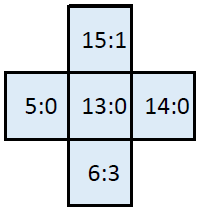
\includegraphics[width=\linewidth]{images/corolle_ex_orientee_3}
			\caption{Exemple de corolle de hamming 1 en $(1,5)$}
			\label{fig:corolle_ex_orientee_3}
		\end{figure}
	\end{minipage}\hfill
		
		
	Sous forme de texte, en excluant la frontière on à donc :
	\begin{lstlisting}
13:1;15:2;14:1; 6:0; 5:1|...
13:1; 5:2;15:3;14:2; 6:1|...
13:1; 6:2; 5:3;15:0;14:3|...
13:1;14:0; 6:3; 5:0;15:1|...
	\end{lstlisting}
	
	On remarque que les 4 dernières pièces (appartenant au hamming 1) bouclent en se décalent de 1 à chaque fois (d'où le fait de \enquote{shifter} les cases).
\end{exmp}

Ce comportement marche sur tous les Hammings. Les pièces appartenant au hamming 2 de la corolle \enquote{shiftent} de 2, et ainsi de suite.

Cette action est gérée par \lstinline[language=python]|pieces_shift|  pour les pièces et \lstinline[language=python]|color_shift| pour la frontière.


\subsection{EternityII(smartforce)}

Le code source se trouve sur : \url{https://gitlab.info-ufr.univ-montp2.fr/EternityII/EternityII/commits/feature/framework_refactoring}

Cette application est composée de deux parties :

\begin{itemize}
	\item le core de l'application (le framework)
	\item l'app qui contient les différentes données nécessaires à la résolution
\end{itemize}

Cette application à été mise en place pour plusieurs raisons :
\begin{itemize}
	\item Pouvoir organiser un grand nombre de données
	\item interconnecter les données entre eux pour optimiser la mise à jour des informations
	\item fournir une platforme modulaire afin de pouvoir facilement intégrer de nouvelles données
	\item mettre en place des systèmes de résolutions alternatifs
	\item implémenter facilement et rapidement de nouvelles façon de parcourir l'arbre
\end{itemize}

\subsubsection{Principe}

Avant d'aborder l'implémentation, il est important de comprendre le principe de l'application.

Le framework est décomposé en 4 parties distinctes :

\begin{enumerate}
	\item Les Modèles
	\item Les Contraintes
	\item Le \enquote{PathFinder}
	\item Le Solveur
\end{enumerate}


\paragraph{Les contraintes}

Les modèles sont contraints par les contraintes, ceux-ci sont chargés de la propagation des données entre les modèles.

\paragraph{Les modèles}

Un modèle est un objet chargé de la manipulation d'une donnée lors de la résolution du problème. Il avertit les modèles auquel il est connecté lors d'un changement utile dans ses données via les contraintes.

\paragraph{Le Pathfinder}

Le PathFinder est connecté à des modèles de référence. Grâce à eux, il détermine le choix de valeur et le choix de variable.

\paragraph{Le solveur}

Le solveur progresse dans l'arbre, à chaque n\oe ud il récupère grâce au PathFinder le n\oe ud suivant à atteindre. Il envoie ensuite la décision aux modèles de références. Si le Pathfinder n'en trouve pas, il envoie alors un ordre de rollback vers le n\oe ud précédent.
\newpage

\subsubsection{Fonctionnement}

\paragraph{Solveur et PathFinder}

Le \textbf{solveur} à un rôle simple, c'est celui qui donne l'ordre de continuer ou non, c'est aussi celui qui est chargé de parcourir l'arbre des possibilités.
Il utilise les ordres suivants :

\begin{description}
	\item [resolve] qui lance la résolution du problème
	\item [resolve(profondeur)] qui détermine le choix de variable (utilise le pathfinder)
	\item [resolve(variable, profondeur)] teste récursivement toutes les valeurs et rappelle \lstinline[language=c++]|resolve(profondeur+1)|. \`{A} la fin de résolution des noeuds fils, un rollback partiel est effectué (on dénie le n\oe ud fils qui vient de se terminer).
	Une fois que toutes les valeurs ont été testés pour la variable actuelle, on fait un rollback total pour revenir au n\oe uds parent (qui déniera le n\oe uds actuel comme choix de variable).
\end{description}

Il contient deux modèles qui sont les points d'entrée vers les autres modèles. C'est à ces deux modèles que les données relatives aux choix de variable et de valeur vont être envoyées.

\begin{figure}[H]
\centering
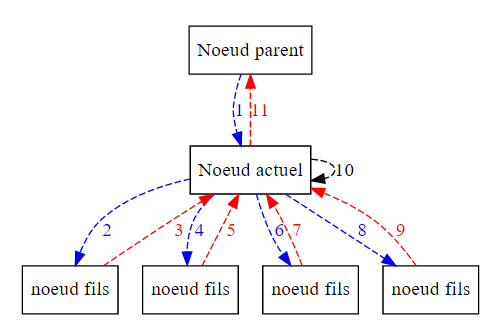
\includegraphics[width=\linewidth]{images/parcours_noeuds}
\caption[Fonctionnement d'un solveur]{Fonctionnement d'un solveur.\\	
	 En bleu, la progression d'un noeud à l'autre.\\ En rouge, un rollback partiel. \\ En noir, un rollback total.\\}
\label{fig:parcoursnoeuds}
\end{figure}

Le \textbf{pathfinder} aide le solveur à prendre des décisions. Il est associés à classes, l'un pour le choix de variable (ex: cases en rowscan), l'autre pour le choix de valeur (ex: pièces en lexico). Il contient 4 ordres :
\begin{description}
	\item [hasNextVariable] qui renvoi vrai s'il existe une variable à une profondeur donnée.
	\item [nextVariable] qui renvoi une variable suivant la stratégie de variable utilisée.
	\item[hasNextValue] renvoi vrai s'il existe une valeur à la variable et la profondeur actuelle
	\item[nextValue] renvoi une valeur suivant la stratégie de utilisée.
\end{description}

Il est important de noter que le pathfinder et le solveur doivent utiliser les mêmes données pour les valeurs et variables, lorsque ceux-ci sont envoyés aux modèles.

\begin{exmp}
	Afin d'éviter, par exemple, d'envoyer les identifiants de BoCo à un solveur CaPi.
\end{exmp}

\subsubsection{Modèles et contraintes}

Les modèles sont interconnectés entre eux grâce aux contraintes.

\begin{figure}[H]
	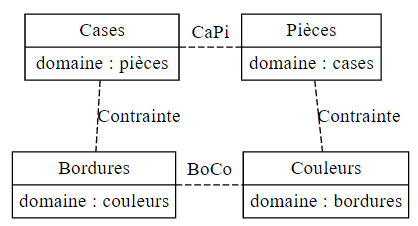
\includegraphics[width=\linewidth]{images/modeles_contraintes}
	\caption{Structure des modèles et des contraintes pour EternityII}
	\label{fig:modeles_contraintes}
\end{figure}

Chaque modèle doit pouvoir effectuer ces actions :

\begin{description}
	\item[allow] autorise un couple de données (ex : CaPi) en tant que variable et valeur pour le n\oe ud actuel. Cela déclenche 2 actions : 
	\begin{itemize}
		\item dénie toutes les autres valeurs pour la variable et réciproquement.
		\item propage l'autorisation du couple aux autres modèles.
	\end{itemize}
	\item[denyOne] dénie le couple de valeur/variable pour la donnée actuelle. on peux aussi dénier définitivement un couple (utile lors d'un parcours en largeur de l'arbre).
	\item[addOne] Utilisé lors de l'initialisation, il permet d'ajouter des données
	\item[rollback(profondeur, total/partiel)] permet de rétablir le modèle à une profondeur antérieure partiellement ou totalement.
\end{description}
\newpage

\subsubsection{Fonctionnement global}

L'ensemble des éléments est gérée par la classe EternityII, elle est aussi chargée de l'hébergement de tous les autres objets.

\begin{figure}[H]
\centering
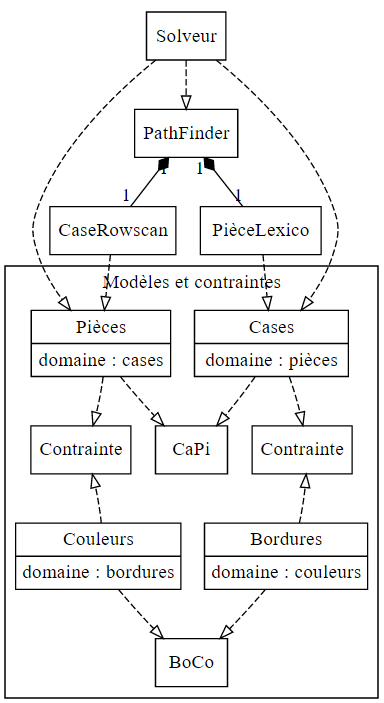
\includegraphics{images/model_simplifie}
\caption{Modèle simplifié du fonctionnement du framework}
\label{fig:model_simplifie}
\end{figure}

Le solveur demande et envoie le couple CaPi depuis le pathfinder aux modèles d'entrées (CaPi), ceux-ci sont chargés de propager l'information aux autres modèles via les contraintes.

\subsubsection{Conseils pour le développement de l'application}

Tout solveur doit hériter de core/SolverInterface.h

Tout choix de variable doit implémenter VariableInterface

Tout choix de valeur doit implémenter ValueInterface

Toute contrainte doit implémenter ConstraintInterface

Tout modèle doit implémenter ModelInterface

Toute donnée transmise d'une classe à l'autre doit implémenter DataInterface

La création de toutes les classes ont lieu dans \lstinline[language=c++]|EternityII::bootstrap|

Tous les fichiers liées à l'application doivent se trouver dans le dossier app/.

Certains commentaires sont à lire lors de toute modification, ils sont préfixés par différents mots-clés :

\begin{description}
	\item[unused :] la fonction n'est pas utilisée
	\item[entrypoint :] lire le commentaire si le point d'entrée à changé
	\item[minimal importance :] La tache à faire n'est pas indispensable au fonctionnement de l'application
	\item[advice :] indique la marche à suivre
	\item[dangerous :] la fonction ou l'algorithme est fragile (dangereuse à utiliser ou a modifier).
\end{description}